\section{Ken Nataro}\label{ken-nataro}
\section{Ken Nataro}\label{ken-nataro-1}


\begin{figure}
\centering
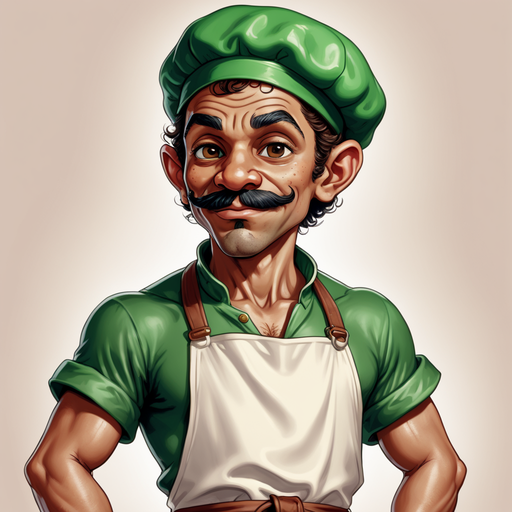
\includegraphics{create-a-digital-illustration-of-ken-nataro-a-mulatto-skinned-halfling-with-a-sturdy-physique-ken--7.png}
\caption{create-a-digital-illustration-of-ken-nataro-a-mulatto-skinned-halfling-with-a-sturdy-physique-ken--7.png}
\end{figure}

Informazioni Generali

Età: 59

Data di nascita: 20/04/1964

Luogo di nascita: Kos

Razza: Halfling

Relazioni: Sposato con Balorca

Alleati: Gilda dei protettori

Alias: U furnaru

Professione: Panettiere


\subsection{Descrizione Generale}\label{descrizione-generale}


\begin{figure}
\centering
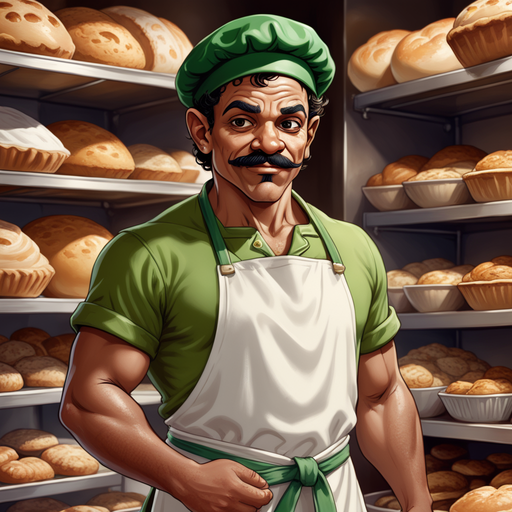
\includegraphics{create-a-digital-illustration-of-ken-nataro-a-mulatto-skinned-halfling-with-a-sturdy-physique-ken--9.png}
\caption{create-a-digital-illustration-of-ken-nataro-a-mulatto-skinned-halfling-with-a-sturdy-physique-ken--9.png}
\end{figure}

Ken Nataro è un halfling di anni con un aspetto insolito per la sua
razza. È dotato di potenti braccia muscolose, frutto di anni e anni di
duro lavoro nella sua panetteria ``da Nataro''. La sua pelle è
abbronzata dal sole e il suo viso mostra rughe di esperienza e di vita
vissuta. I suoi occhi sono vivaci e riflettono la profonda ira che
cresce in lui quando si trova di fronte all'ingiustizia.

\subsection{Biografia}\label{biografia}


\subsubsection{Infanzia}\label{infanzia}

Ken Nataro è nato in una famiglia di panettieri halfling con una
tradizione secolare di produzione del pane. Fin da piccolo, Ken mostrava
un interesse vivace per il mestiere di famiglia. Mentre i suoi coetanei
giocavano a nascondino, Ken preferiva impastare la pasta e osservare il
pane lievitare nel forno a legna. La panetteria ``da Nataro'' era il
cuore pulsante della comunità halfling di Kos, e Ken amava passare il
tempo con i suoi genitori e i suoi nonni mentre apprendeva i segreti
dell'arte della panificazione.

\subsubsection{\texorpdfstring{\textbf{Eredità della
Panetteria}}{Eredità della Panetteria}}\label{eredituxe0-della-panetteria}

All'età di anni, dopo anni di apprendistato e duro lavoro nella
panetteria di famiglia, Ken ereditò ufficialmente la gestione della
panetteria ``da Nataro'' dai suoi genitori. Questo fu un momento di
grande responsabilità, ma anche di orgoglio per Ken, che si sentiva
onorato nel portare avanti la tradizione familiare. La panetteria era
famosa in tutta Kos per il suo pane fragrante e le sue prelibatezze da
forno, che erano richieste persino dai nobili di Kos durante le
festività.

\subsubsection{\texorpdfstring{\textbf{La Lenta
Decadenza}}{La Lenta Decadenza}}\label{la-lenta-decadenza}

Nonostante il suo impegno instancabile e il desiderio di preservare la
gloria della panetteria, Ken dovette affrontare tempi difficili. I
cambiamenti nel commercio del grano e le fluttuazioni economiche in Kos
iniziarono a colpire la sua attività. La panetteria ``da Nataro'' non
era più la potenza economica di un tempo, e Ken faticava a mantenere i
livelli di produzione e a sbarcare il lunario. Questi tempi difficili
fecero emergere in lui la sua innata ira e desiderio di ristabilire
l'equilibrio nella sua vita.

\subsubsection{\texorpdfstring{Entrata ne\textbf{lla Gilda dei
Protettori}}{Entrata nella Gilda dei Protettori}}\label{entrata-nella-gilda-dei-protettori}

Per affrontare le crescenti difficoltà finanziarie e sostenere la sua
numerosa famiglia, Ken prese una decisione radicale. All'età di anni,
lasciò la gestione quotidiana della panetteria nelle mani di sua moglie,
Balorca, una mezz'orca dal cuore gentile, e decise di unirsi alla Gilda
dei Protettori. Questa decisione fu dettata dalla necessità di
guadagnare un reddito extra, ma anche dalla sua crescente ira per le
ingiustizie del mondo. Ken trasformò la sua rabbia in una forza
formidabile nel campo di battaglia, diventando un membro valoroso della
gilda. Oggi, Ken Nataro bilancia la sua vita da panettiere con le sue
nuove avventure come barbaro nella Gilda dei Protettori. La sua
dedizione alla sua famiglia, la sua passione per la panificazione e il
suo desiderio di giustizia sono i pilastri della sua vita, rendendolo un
personaggio complesso e affascinante nel mondo di Kos.

\subsection{Personalità}\label{personalituxe0}


Ken Nataro è un individuo di straordinaria forza d'animo e
determinazione. La sua personalità è caratterizzata da un profondo senso
di responsabilità e un attaccamento radicato alla sua famiglia e alla
sua tradizione. È gentile e affettuoso con i suoi dieci figli, e la sua
relazione con sua moglie, Balorca, è fondata su un amore profondo e una
profonda comprensione reciproca.

Tuttavia, sotto la superficie calma e affettuosa, alberga una fiamma di
ira ardente. Le ingiustizie del mondo, in particolare quelle che hanno
colpito la sua amata panetteria di famiglia, alimentano la sua
determinazione a fare del bene e a ristabilire l'equilibrio. Quando si
trova di fronte all'ingiustizia o alla crudeltà, questa ira si trasforma
in una forza indomabile che lo guida in battaglia, conferendo a Ken un
coraggio straordinario e una capacità di combattimento formidabile.

Ken è anche noto per la sua generosità e la sua propensione a sostenere
chi è in difficoltà, e questo lo rende un membro prezioso della Gilda
dei Protettori. È sempre pronto a tendere una mano agli amici e agli
alleati e a difendere coloro che non possono difendersi da soli. La sua
personalità complessa, con una mescolanza di gentilezza, ira e spirito
combattivo, lo rende un personaggio affascinante e un alleato fidato
nelle avventure di Kos

\subsection{Coinvolgimenti in eventi
recenti}\label{coinvolgimenti-in-eventi-recenti}


\href{Untitled\%206d32341cd290432098378da8e9e19b98.csv}{}

